\documentclass[margin=2mm]{standalone}
\usepackage{tikz}
\usepackage{amsmath,amssymb,mathtools}
\begin{document}
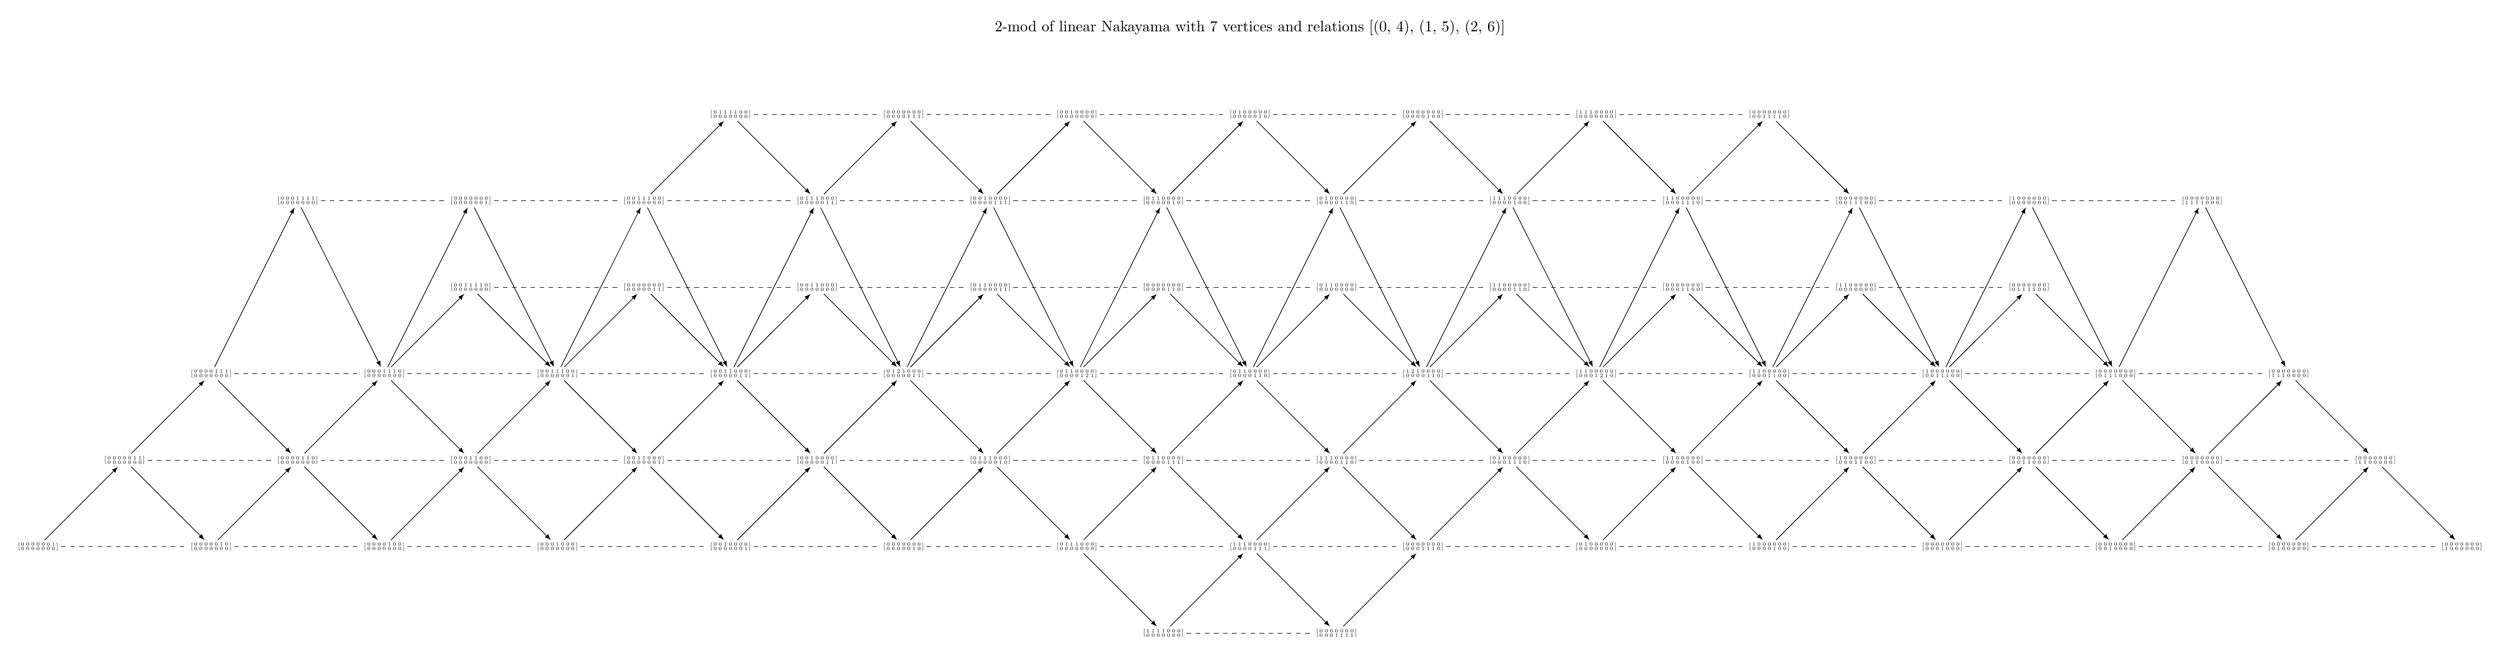
\begin{tikzpicture}[xscale=2,yscale=2]
\node at (14.0,6) [] {$2$-mod of linear Nakayama with 7 vertices and relations [(0, 4), (1, 5), (2, 6)]};
\node (t-0P0) at (13,-1) [scale=0.5] {$\begin{bsmallmatrix}
 1 & 1 & 1 & 1 & 0 & 0 & 0\\
 0 & 0 & 0 & 0 & 0 & 0 & 0\\
\end{bsmallmatrix}$};
\node (t-1P0) at (15,-1) [scale=0.5] {$\begin{bsmallmatrix}
 0 & 0 & 0 & 0 & 0 & 0 & 0\\
 0 & 0 & 0 & 1 & 1 & 1 & 1\\
\end{bsmallmatrix}$};
\node (t-0P1) at (8,5) [scale=0.5] {$\begin{bsmallmatrix}
 0 & 1 & 1 & 1 & 1 & 0 & 0\\
 0 & 0 & 0 & 0 & 0 & 0 & 0\\
\end{bsmallmatrix}$};
\node (t-1P1) at (10,5) [scale=0.5] {$\begin{bsmallmatrix}
 0 & 0 & 0 & 0 & 0 & 0 & 0\\
 0 & 0 & 0 & 0 & 1 & 1 & 1\\
\end{bsmallmatrix}$};
\node (t-2P1) at (12,5) [scale=0.5] {$\begin{bsmallmatrix}
 0 & 0 & 1 & 0 & 0 & 0 & 0\\
 0 & 0 & 0 & 0 & 0 & 0 & 0\\
\end{bsmallmatrix}$};
\node (t-3P1) at (14,5) [scale=0.5] {$\begin{bsmallmatrix}
 0 & 1 & 0 & 0 & 0 & 0 & 0\\
 0 & 0 & 0 & 0 & 0 & 1 & 0\\
\end{bsmallmatrix}$};
\node (t-4P1) at (16,5) [scale=0.5] {$\begin{bsmallmatrix}
 0 & 0 & 0 & 0 & 0 & 0 & 0\\
 0 & 0 & 0 & 0 & 1 & 0 & 0\\
\end{bsmallmatrix}$};
\node (t-5P1) at (18,5) [scale=0.5] {$\begin{bsmallmatrix}
 1 & 1 & 1 & 0 & 0 & 0 & 0\\
 0 & 0 & 0 & 0 & 0 & 0 & 0\\
\end{bsmallmatrix}$};
\node (t-6P1) at (20,5) [scale=0.5] {$\begin{bsmallmatrix}
 0 & 0 & 0 & 0 & 0 & 0 & 0\\
 0 & 0 & 1 & 1 & 1 & 1 & 0\\
\end{bsmallmatrix}$};
\node (t-0P2) at (5,3) [scale=0.5] {$\begin{bsmallmatrix}
 0 & 0 & 1 & 1 & 1 & 1 & 0\\
 0 & 0 & 0 & 0 & 0 & 0 & 0\\
\end{bsmallmatrix}$};
\node (t-1P2) at (7,3) [scale=0.5] {$\begin{bsmallmatrix}
 0 & 0 & 0 & 0 & 0 & 0 & 0\\
 0 & 0 & 0 & 0 & 0 & 1 & 1\\
\end{bsmallmatrix}$};
\node (t-2P2) at (9,3) [scale=0.5] {$\begin{bsmallmatrix}
 0 & 0 & 1 & 1 & 0 & 0 & 0\\
 0 & 0 & 0 & 0 & 0 & 0 & 0\\
\end{bsmallmatrix}$};
\node (t-3P2) at (11,3) [scale=0.5] {$\begin{bsmallmatrix}
 0 & 1 & 1 & 0 & 0 & 0 & 0\\
 0 & 0 & 0 & 0 & 0 & 1 & 1\\
\end{bsmallmatrix}$};
\node (t-4P2) at (13,3) [scale=0.5] {$\begin{bsmallmatrix}
 0 & 0 & 0 & 0 & 0 & 0 & 0\\
 0 & 0 & 0 & 0 & 1 & 1 & 0\\
\end{bsmallmatrix}$};
\node (t-5P2) at (15,3) [scale=0.5] {$\begin{bsmallmatrix}
 0 & 1 & 1 & 0 & 0 & 0 & 0\\
 0 & 0 & 0 & 0 & 0 & 0 & 0\\
\end{bsmallmatrix}$};
\node (t-6P2) at (17,3) [scale=0.5] {$\begin{bsmallmatrix}
 1 & 1 & 0 & 0 & 0 & 0 & 0\\
 0 & 0 & 0 & 0 & 1 & 1 & 0\\
\end{bsmallmatrix}$};
\node (t-7P2) at (19,3) [scale=0.5] {$\begin{bsmallmatrix}
 0 & 0 & 0 & 0 & 0 & 0 & 0\\
 0 & 0 & 0 & 1 & 1 & 0 & 0\\
\end{bsmallmatrix}$};
\node (t-8P2) at (21,3) [scale=0.5] {$\begin{bsmallmatrix}
 1 & 1 & 0 & 0 & 0 & 0 & 0\\
 0 & 0 & 0 & 0 & 0 & 0 & 0\\
\end{bsmallmatrix}$};
\node (t-9P2) at (23,3) [scale=0.5] {$\begin{bsmallmatrix}
 0 & 0 & 0 & 0 & 0 & 0 & 0\\
 0 & 1 & 1 & 1 & 1 & 0 & 0\\
\end{bsmallmatrix}$};
\node (t-0P3) at (3,4) [scale=0.5] {$\begin{bsmallmatrix}
 0 & 0 & 0 & 1 & 1 & 1 & 1\\
 0 & 0 & 0 & 0 & 0 & 0 & 0\\
\end{bsmallmatrix}$};
\node (t-1P3) at (5,4) [scale=0.5] {$\begin{bsmallmatrix}
 0 & 0 & 0 & 0 & 0 & 0 & 0\\
 0 & 0 & 0 & 0 & 0 & 0 & 1\\
\end{bsmallmatrix}$};
\node (t-2P3) at (7,4) [scale=0.5] {$\begin{bsmallmatrix}
 0 & 0 & 1 & 1 & 1 & 0 & 0\\
 0 & 0 & 0 & 0 & 0 & 0 & 0\\
\end{bsmallmatrix}$};
\node (t-3P3) at (9,4) [scale=0.5] {$\begin{bsmallmatrix}
 0 & 1 & 1 & 1 & 0 & 0 & 0\\
 0 & 0 & 0 & 0 & 0 & 1 & 1\\
\end{bsmallmatrix}$};
\node (t-4P3) at (11,4) [scale=0.5] {$\begin{bsmallmatrix}
 0 & 0 & 1 & 0 & 0 & 0 & 0\\
 0 & 0 & 0 & 0 & 1 & 1 & 1\\
\end{bsmallmatrix}$};
\node (t-5P3) at (13,4) [scale=0.5] {$\begin{bsmallmatrix}
 0 & 1 & 1 & 0 & 0 & 0 & 0\\
 0 & 0 & 0 & 0 & 0 & 1 & 0\\
\end{bsmallmatrix}$};
\node (t-6P3) at (15,4) [scale=0.5] {$\begin{bsmallmatrix}
 0 & 1 & 0 & 0 & 0 & 0 & 0\\
 0 & 0 & 0 & 0 & 1 & 1 & 0\\
\end{bsmallmatrix}$};
\node (t-7P3) at (17,4) [scale=0.5] {$\begin{bsmallmatrix}
 1 & 1 & 1 & 0 & 0 & 0 & 0\\
 0 & 0 & 0 & 0 & 1 & 0 & 0\\
\end{bsmallmatrix}$};
\node (t-8P3) at (19,4) [scale=0.5] {$\begin{bsmallmatrix}
 1 & 1 & 0 & 0 & 0 & 0 & 0\\
 0 & 0 & 0 & 1 & 1 & 1 & 0\\
\end{bsmallmatrix}$};
\node (t-9P3) at (21,4) [scale=0.5] {$\begin{bsmallmatrix}
 0 & 0 & 0 & 0 & 0 & 0 & 0\\
 0 & 0 & 1 & 1 & 1 & 0 & 0\\
\end{bsmallmatrix}$};
\node (t-10P3) at (23,4) [scale=0.5] {$\begin{bsmallmatrix}
 1 & 0 & 0 & 0 & 0 & 0 & 0\\
 0 & 0 & 0 & 0 & 0 & 0 & 0\\
\end{bsmallmatrix}$};
\node (t-11P3) at (25,4) [scale=0.5] {$\begin{bsmallmatrix}
 0 & 0 & 0 & 0 & 0 & 0 & 0\\
 1 & 1 & 1 & 1 & 0 & 0 & 0\\
\end{bsmallmatrix}$};
\node (t-0P4) at (2,2) [scale=0.5] {$\begin{bsmallmatrix}
 0 & 0 & 0 & 0 & 1 & 1 & 1\\
 0 & 0 & 0 & 0 & 0 & 0 & 0\\
\end{bsmallmatrix}$};
\node (t-1P4) at (4,2) [scale=0.5] {$\begin{bsmallmatrix}
 0 & 0 & 0 & 1 & 1 & 1 & 0\\
 0 & 0 & 0 & 0 & 0 & 0 & 0\\
\end{bsmallmatrix}$};
\node (t-2P4) at (6,2) [scale=0.5] {$\begin{bsmallmatrix}
 0 & 0 & 1 & 1 & 1 & 0 & 0\\
 0 & 0 & 0 & 0 & 0 & 0 & 1\\
\end{bsmallmatrix}$};
\node (t-3P4) at (8,2) [scale=0.5] {$\begin{bsmallmatrix}
 0 & 0 & 1 & 1 & 0 & 0 & 0\\
 0 & 0 & 0 & 0 & 0 & 1 & 1\\
\end{bsmallmatrix}$};
\node (t-4P4) at (10,2) [scale=0.5] {$\begin{bsmallmatrix}
 0 & 1 & 2 & 1 & 0 & 0 & 0\\
 0 & 0 & 0 & 0 & 0 & 1 & 1\\
\end{bsmallmatrix}$};
\node (t-5P4) at (12,2) [scale=0.5] {$\begin{bsmallmatrix}
 0 & 1 & 1 & 0 & 0 & 0 & 0\\
 0 & 0 & 0 & 0 & 1 & 2 & 1\\
\end{bsmallmatrix}$};
\node (t-6P4) at (14,2) [scale=0.5] {$\begin{bsmallmatrix}
 0 & 1 & 1 & 0 & 0 & 0 & 0\\
 0 & 0 & 0 & 0 & 1 & 1 & 0\\
\end{bsmallmatrix}$};
\node (t-7P4) at (16,2) [scale=0.5] {$\begin{bsmallmatrix}
 1 & 2 & 1 & 0 & 0 & 0 & 0\\
 0 & 0 & 0 & 0 & 1 & 1 & 0\\
\end{bsmallmatrix}$};
\node (t-8P4) at (18,2) [scale=0.5] {$\begin{bsmallmatrix}
 1 & 1 & 0 & 0 & 0 & 0 & 0\\
 0 & 0 & 0 & 1 & 2 & 1 & 0\\
\end{bsmallmatrix}$};
\node (t-9P4) at (20,2) [scale=0.5] {$\begin{bsmallmatrix}
 1 & 1 & 0 & 0 & 0 & 0 & 0\\
 0 & 0 & 0 & 1 & 1 & 0 & 0\\
\end{bsmallmatrix}$};
\node (t-10P4) at (22,2) [scale=0.5] {$\begin{bsmallmatrix}
 1 & 0 & 0 & 0 & 0 & 0 & 0\\
 0 & 0 & 1 & 1 & 1 & 0 & 0\\
\end{bsmallmatrix}$};
\node (t-11P4) at (24,2) [scale=0.5] {$\begin{bsmallmatrix}
 0 & 0 & 0 & 0 & 0 & 0 & 0\\
 0 & 1 & 1 & 1 & 0 & 0 & 0\\
\end{bsmallmatrix}$};
\node (t-12P4) at (26,2) [scale=0.5] {$\begin{bsmallmatrix}
 0 & 0 & 0 & 0 & 0 & 0 & 0\\
 1 & 1 & 1 & 0 & 0 & 0 & 0\\
\end{bsmallmatrix}$};
\node (t-0P5) at (1,1) [scale=0.5] {$\begin{bsmallmatrix}
 0 & 0 & 0 & 0 & 0 & 1 & 1\\
 0 & 0 & 0 & 0 & 0 & 0 & 0\\
\end{bsmallmatrix}$};
\node (t-1P5) at (3,1) [scale=0.5] {$\begin{bsmallmatrix}
 0 & 0 & 0 & 0 & 1 & 1 & 0\\
 0 & 0 & 0 & 0 & 0 & 0 & 0\\
\end{bsmallmatrix}$};
\node (t-2P5) at (5,1) [scale=0.5] {$\begin{bsmallmatrix}
 0 & 0 & 0 & 1 & 1 & 0 & 0\\
 0 & 0 & 0 & 0 & 0 & 0 & 0\\
\end{bsmallmatrix}$};
\node (t-3P5) at (7,1) [scale=0.5] {$\begin{bsmallmatrix}
 0 & 0 & 1 & 1 & 0 & 0 & 0\\
 0 & 0 & 0 & 0 & 0 & 0 & 1\\
\end{bsmallmatrix}$};
\node (t-4P5) at (9,1) [scale=0.5] {$\begin{bsmallmatrix}
 0 & 0 & 1 & 0 & 0 & 0 & 0\\
 0 & 0 & 0 & 0 & 0 & 1 & 1\\
\end{bsmallmatrix}$};
\node (t-5P5) at (11,1) [scale=0.5] {$\begin{bsmallmatrix}
 0 & 1 & 1 & 1 & 0 & 0 & 0\\
 0 & 0 & 0 & 0 & 0 & 1 & 0\\
\end{bsmallmatrix}$};
\node (t-6P5) at (13,1) [scale=0.5] {$\begin{bsmallmatrix}
 0 & 1 & 1 & 0 & 0 & 0 & 0\\
 0 & 0 & 0 & 0 & 1 & 1 & 1\\
\end{bsmallmatrix}$};
\node (t-7P5) at (15,1) [scale=0.5] {$\begin{bsmallmatrix}
 1 & 1 & 1 & 0 & 0 & 0 & 0\\
 0 & 0 & 0 & 0 & 1 & 1 & 0\\
\end{bsmallmatrix}$};
\node (t-8P5) at (17,1) [scale=0.5] {$\begin{bsmallmatrix}
 0 & 1 & 0 & 0 & 0 & 0 & 0\\
 0 & 0 & 0 & 1 & 1 & 1 & 0\\
\end{bsmallmatrix}$};
\node (t-9P5) at (19,1) [scale=0.5] {$\begin{bsmallmatrix}
 1 & 1 & 0 & 0 & 0 & 0 & 0\\
 0 & 0 & 0 & 0 & 1 & 0 & 0\\
\end{bsmallmatrix}$};
\node (t-10P5) at (21,1) [scale=0.5] {$\begin{bsmallmatrix}
 1 & 0 & 0 & 0 & 0 & 0 & 0\\
 0 & 0 & 0 & 1 & 1 & 0 & 0\\
\end{bsmallmatrix}$};
\node (t-11P5) at (23,1) [scale=0.5] {$\begin{bsmallmatrix}
 0 & 0 & 0 & 0 & 0 & 0 & 0\\
 0 & 0 & 1 & 1 & 0 & 0 & 0\\
\end{bsmallmatrix}$};
\node (t-12P5) at (25,1) [scale=0.5] {$\begin{bsmallmatrix}
 0 & 0 & 0 & 0 & 0 & 0 & 0\\
 0 & 1 & 1 & 0 & 0 & 0 & 0\\
\end{bsmallmatrix}$};
\node (t-13P5) at (27,1) [scale=0.5] {$\begin{bsmallmatrix}
 0 & 0 & 0 & 0 & 0 & 0 & 0\\
 1 & 1 & 0 & 0 & 0 & 0 & 0\\
\end{bsmallmatrix}$};
\node (t-0P6) at (0,0) [scale=0.5] {$\begin{bsmallmatrix}
 0 & 0 & 0 & 0 & 0 & 0 & 1\\
 0 & 0 & 0 & 0 & 0 & 0 & 0\\
\end{bsmallmatrix}$};
\node (t-1P6) at (2,0) [scale=0.5] {$\begin{bsmallmatrix}
 0 & 0 & 0 & 0 & 0 & 1 & 0\\
 0 & 0 & 0 & 0 & 0 & 0 & 0\\
\end{bsmallmatrix}$};
\node (t-2P6) at (4,0) [scale=0.5] {$\begin{bsmallmatrix}
 0 & 0 & 0 & 0 & 1 & 0 & 0\\
 0 & 0 & 0 & 0 & 0 & 0 & 0\\
\end{bsmallmatrix}$};
\node (t-3P6) at (6,0) [scale=0.5] {$\begin{bsmallmatrix}
 0 & 0 & 0 & 1 & 0 & 0 & 0\\
 0 & 0 & 0 & 0 & 0 & 0 & 0\\
\end{bsmallmatrix}$};
\node (t-4P6) at (8,0) [scale=0.5] {$\begin{bsmallmatrix}
 0 & 0 & 1 & 0 & 0 & 0 & 0\\
 0 & 0 & 0 & 0 & 0 & 0 & 1\\
\end{bsmallmatrix}$};
\node (t-5P6) at (10,0) [scale=0.5] {$\begin{bsmallmatrix}
 0 & 0 & 0 & 0 & 0 & 0 & 0\\
 0 & 0 & 0 & 0 & 0 & 1 & 0\\
\end{bsmallmatrix}$};
\node (t-6P6) at (12,0) [scale=0.5] {$\begin{bsmallmatrix}
 0 & 1 & 1 & 1 & 0 & 0 & 0\\
 0 & 0 & 0 & 0 & 0 & 0 & 0\\
\end{bsmallmatrix}$};
\node (t-7P6) at (14,0) [scale=0.5] {$\begin{bsmallmatrix}
 1 & 1 & 1 & 0 & 0 & 0 & 0\\
 0 & 0 & 0 & 0 & 1 & 1 & 1\\
\end{bsmallmatrix}$};
\node (t-8P6) at (16,0) [scale=0.5] {$\begin{bsmallmatrix}
 0 & 0 & 0 & 0 & 0 & 0 & 0\\
 0 & 0 & 0 & 1 & 1 & 1 & 0\\
\end{bsmallmatrix}$};
\node (t-9P6) at (18,0) [scale=0.5] {$\begin{bsmallmatrix}
 0 & 1 & 0 & 0 & 0 & 0 & 0\\
 0 & 0 & 0 & 0 & 0 & 0 & 0\\
\end{bsmallmatrix}$};
\node (t-10P6) at (20,0) [scale=0.5] {$\begin{bsmallmatrix}
 1 & 0 & 0 & 0 & 0 & 0 & 0\\
 0 & 0 & 0 & 0 & 1 & 0 & 0\\
\end{bsmallmatrix}$};
\node (t-11P6) at (22,0) [scale=0.5] {$\begin{bsmallmatrix}
 0 & 0 & 0 & 0 & 0 & 0 & 0\\
 0 & 0 & 0 & 1 & 0 & 0 & 0\\
\end{bsmallmatrix}$};
\node (t-12P6) at (24,0) [scale=0.5] {$\begin{bsmallmatrix}
 0 & 0 & 0 & 0 & 0 & 0 & 0\\
 0 & 0 & 1 & 0 & 0 & 0 & 0\\
\end{bsmallmatrix}$};
\node (t-13P6) at (26,0) [scale=0.5] {$\begin{bsmallmatrix}
 0 & 0 & 0 & 0 & 0 & 0 & 0\\
 0 & 1 & 0 & 0 & 0 & 0 & 0\\
\end{bsmallmatrix}$};
\node (t-14P6) at (28,0) [scale=0.5] {$\begin{bsmallmatrix}
 0 & 0 & 0 & 0 & 0 & 0 & 0\\
 1 & 0 & 0 & 0 & 0 & 0 & 0\\
\end{bsmallmatrix}$};
\draw[-latex] (t-0P0) -- (t-7P6);
\draw[-latex] (t-1P0) -- (t-8P6);
\draw[-latex] (t-0P1) -- (t-3P3);
\draw[-latex] (t-1P1) -- (t-4P3);
\draw[-latex] (t-2P1) -- (t-5P3);
\draw[-latex] (t-3P1) -- (t-6P3);
\draw[-latex] (t-4P1) -- (t-7P3);
\draw[-latex] (t-5P1) -- (t-8P3);
\draw[-latex] (t-6P1) -- (t-9P3);
\draw[-latex] (t-0P2) -- (t-2P4);
\draw[-latex] (t-1P2) -- (t-3P4);
\draw[-latex] (t-2P2) -- (t-4P4);
\draw[-latex] (t-3P2) -- (t-5P4);
\draw[-latex] (t-4P2) -- (t-6P4);
\draw[-latex] (t-5P2) -- (t-7P4);
\draw[-latex] (t-6P2) -- (t-8P4);
\draw[-latex] (t-7P2) -- (t-9P4);
\draw[-latex] (t-8P2) -- (t-10P4);
\draw[-latex] (t-9P2) -- (t-11P4);
\draw[-latex] (t-0P3) -- (t-1P4);
\draw[-latex] (t-1P3) -- (t-2P4);
\draw[-latex] (t-2P3) -- (t-0P1);
\draw[-latex] (t-2P3) -- (t-3P4);
\draw[-latex] (t-3P3) -- (t-4P4);
\draw[-latex] (t-3P3) -- (t-1P1);
\draw[-latex] (t-4P3) -- (t-5P4);
\draw[-latex] (t-4P3) -- (t-2P1);
\draw[-latex] (t-5P3) -- (t-6P4);
\draw[-latex] (t-5P3) -- (t-3P1);
\draw[-latex] (t-6P3) -- (t-7P4);
\draw[-latex] (t-6P3) -- (t-4P1);
\draw[-latex] (t-7P3) -- (t-8P4);
\draw[-latex] (t-7P3) -- (t-5P1);
\draw[-latex] (t-8P3) -- (t-9P4);
\draw[-latex] (t-8P3) -- (t-6P1);
\draw[-latex] (t-9P3) -- (t-10P4);
\draw[-latex] (t-10P3) -- (t-11P4);
\draw[-latex] (t-11P3) -- (t-12P4);
\draw[-latex] (t-0P4) -- (t-0P3);
\draw[-latex] (t-0P4) -- (t-1P5);
\draw[-latex] (t-1P4) -- (t-0P2);
\draw[-latex] (t-1P4) -- (t-1P3);
\draw[-latex] (t-1P4) -- (t-2P5);
\draw[-latex] (t-2P4) -- (t-1P2);
\draw[-latex] (t-2P4) -- (t-2P3);
\draw[-latex] (t-2P4) -- (t-3P5);
\draw[-latex] (t-3P4) -- (t-2P2);
\draw[-latex] (t-3P4) -- (t-3P3);
\draw[-latex] (t-3P4) -- (t-4P5);
\draw[-latex] (t-4P4) -- (t-3P2);
\draw[-latex] (t-4P4) -- (t-4P3);
\draw[-latex] (t-4P4) -- (t-5P5);
\draw[-latex] (t-5P4) -- (t-4P2);
\draw[-latex] (t-5P4) -- (t-5P3);
\draw[-latex] (t-5P4) -- (t-6P5);
\draw[-latex] (t-6P4) -- (t-5P2);
\draw[-latex] (t-6P4) -- (t-6P3);
\draw[-latex] (t-6P4) -- (t-7P5);
\draw[-latex] (t-7P4) -- (t-6P2);
\draw[-latex] (t-7P4) -- (t-7P3);
\draw[-latex] (t-7P4) -- (t-8P5);
\draw[-latex] (t-8P4) -- (t-7P2);
\draw[-latex] (t-8P4) -- (t-8P3);
\draw[-latex] (t-8P4) -- (t-9P5);
\draw[-latex] (t-9P4) -- (t-8P2);
\draw[-latex] (t-9P4) -- (t-9P3);
\draw[-latex] (t-9P4) -- (t-10P5);
\draw[-latex] (t-10P4) -- (t-9P2);
\draw[-latex] (t-10P4) -- (t-10P3);
\draw[-latex] (t-10P4) -- (t-11P5);
\draw[-latex] (t-11P4) -- (t-11P3);
\draw[-latex] (t-11P4) -- (t-12P5);
\draw[-latex] (t-12P4) -- (t-13P5);
\draw[-latex] (t-0P5) -- (t-0P4);
\draw[-latex] (t-0P5) -- (t-1P6);
\draw[-latex] (t-1P5) -- (t-1P4);
\draw[-latex] (t-1P5) -- (t-2P6);
\draw[-latex] (t-2P5) -- (t-2P4);
\draw[-latex] (t-2P5) -- (t-3P6);
\draw[-latex] (t-3P5) -- (t-3P4);
\draw[-latex] (t-3P5) -- (t-4P6);
\draw[-latex] (t-4P5) -- (t-4P4);
\draw[-latex] (t-4P5) -- (t-5P6);
\draw[-latex] (t-5P5) -- (t-5P4);
\draw[-latex] (t-5P5) -- (t-6P6);
\draw[-latex] (t-6P5) -- (t-6P4);
\draw[-latex] (t-6P5) -- (t-7P6);
\draw[-latex] (t-7P5) -- (t-7P4);
\draw[-latex] (t-7P5) -- (t-8P6);
\draw[-latex] (t-8P5) -- (t-8P4);
\draw[-latex] (t-8P5) -- (t-9P6);
\draw[-latex] (t-9P5) -- (t-9P4);
\draw[-latex] (t-9P5) -- (t-10P6);
\draw[-latex] (t-10P5) -- (t-10P4);
\draw[-latex] (t-10P5) -- (t-11P6);
\draw[-latex] (t-11P5) -- (t-11P4);
\draw[-latex] (t-11P5) -- (t-12P6);
\draw[-latex] (t-12P5) -- (t-12P4);
\draw[-latex] (t-12P5) -- (t-13P6);
\draw[-latex] (t-13P5) -- (t-14P6);
\draw[-latex] (t-0P6) -- (t-0P5);
\draw[-latex] (t-1P6) -- (t-1P5);
\draw[-latex] (t-2P6) -- (t-2P5);
\draw[-latex] (t-3P6) -- (t-3P5);
\draw[-latex] (t-4P6) -- (t-4P5);
\draw[-latex] (t-5P6) -- (t-5P5);
\draw[-latex] (t-6P6) -- (t-0P0);
\draw[-latex] (t-6P6) -- (t-6P5);
\draw[-latex] (t-7P6) -- (t-7P5);
\draw[-latex] (t-7P6) -- (t-1P0);
\draw[-latex] (t-8P6) -- (t-8P5);
\draw[-latex] (t-9P6) -- (t-9P5);
\draw[-latex] (t-10P6) -- (t-10P5);
\draw[-latex] (t-11P6) -- (t-11P5);
\draw[-latex] (t-12P6) -- (t-12P5);
\draw[-latex] (t-13P6) -- (t-13P5);
\draw[dashed] (t-0P0)--(t-1P0);
\draw[dashed] (t-0P1)--(t-1P1);
\draw[dashed] (t-1P1)--(t-2P1);
\draw[dashed] (t-2P1)--(t-3P1);
\draw[dashed] (t-3P1)--(t-4P1);
\draw[dashed] (t-4P1)--(t-5P1);
\draw[dashed] (t-5P1)--(t-6P1);
\draw[dashed] (t-0P2)--(t-1P2);
\draw[dashed] (t-1P2)--(t-2P2);
\draw[dashed] (t-2P2)--(t-3P2);
\draw[dashed] (t-3P2)--(t-4P2);
\draw[dashed] (t-4P2)--(t-5P2);
\draw[dashed] (t-5P2)--(t-6P2);
\draw[dashed] (t-6P2)--(t-7P2);
\draw[dashed] (t-7P2)--(t-8P2);
\draw[dashed] (t-8P2)--(t-9P2);
\draw[dashed] (t-0P3)--(t-1P3);
\draw[dashed] (t-1P3)--(t-2P3);
\draw[dashed] (t-2P3)--(t-3P3);
\draw[dashed] (t-3P3)--(t-4P3);
\draw[dashed] (t-4P3)--(t-5P3);
\draw[dashed] (t-5P3)--(t-6P3);
\draw[dashed] (t-6P3)--(t-7P3);
\draw[dashed] (t-7P3)--(t-8P3);
\draw[dashed] (t-8P3)--(t-9P3);
\draw[dashed] (t-9P3)--(t-10P3);
\draw[dashed] (t-10P3)--(t-11P3);
\draw[dashed] (t-0P4)--(t-1P4);
\draw[dashed] (t-1P4)--(t-2P4);
\draw[dashed] (t-2P4)--(t-3P4);
\draw[dashed] (t-3P4)--(t-4P4);
\draw[dashed] (t-4P4)--(t-5P4);
\draw[dashed] (t-5P4)--(t-6P4);
\draw[dashed] (t-6P4)--(t-7P4);
\draw[dashed] (t-7P4)--(t-8P4);
\draw[dashed] (t-8P4)--(t-9P4);
\draw[dashed] (t-9P4)--(t-10P4);
\draw[dashed] (t-10P4)--(t-11P4);
\draw[dashed] (t-11P4)--(t-12P4);
\draw[dashed] (t-0P5)--(t-1P5);
\draw[dashed] (t-1P5)--(t-2P5);
\draw[dashed] (t-2P5)--(t-3P5);
\draw[dashed] (t-3P5)--(t-4P5);
\draw[dashed] (t-4P5)--(t-5P5);
\draw[dashed] (t-5P5)--(t-6P5);
\draw[dashed] (t-6P5)--(t-7P5);
\draw[dashed] (t-7P5)--(t-8P5);
\draw[dashed] (t-8P5)--(t-9P5);
\draw[dashed] (t-9P5)--(t-10P5);
\draw[dashed] (t-10P5)--(t-11P5);
\draw[dashed] (t-11P5)--(t-12P5);
\draw[dashed] (t-12P5)--(t-13P5);
\draw[dashed] (t-0P6)--(t-1P6);
\draw[dashed] (t-1P6)--(t-2P6);
\draw[dashed] (t-2P6)--(t-3P6);
\draw[dashed] (t-3P6)--(t-4P6);
\draw[dashed] (t-4P6)--(t-5P6);
\draw[dashed] (t-5P6)--(t-6P6);
\draw[dashed] (t-6P6)--(t-7P6);
\draw[dashed] (t-7P6)--(t-8P6);
\draw[dashed] (t-8P6)--(t-9P6);
\draw[dashed] (t-9P6)--(t-10P6);
\draw[dashed] (t-10P6)--(t-11P6);
\draw[dashed] (t-11P6)--(t-12P6);
\draw[dashed] (t-12P6)--(t-13P6);
\draw[dashed] (t-13P6)--(t-14P6);
\end{tikzpicture}\end{document}